\chapter{Ideal Gases}\label{ch:ig}

The ideal gas is one in which bombarding molecules do not exert significant forces on each other except in collisions.  Under these conditions, the distance between molecules (the gas's density) is unimportant for determining thermodynamic properties.  Only the gas's temperature (the speed of the molecules) is important.  It is worth emphasizing that transport properties (like conductivity and diffusivity) are still impacted by density.

There are two classes in \PM\ that implement the two most widely used models: the \verb|ig| class manages the Shomate equation of state, and \verb|ig2| manages the so-called NASA polynomials equation of state.  In either case, constant-pressure specific heat, $c_p$, is constructed purely as a function of temperature.  Here, we re-develop the thermodynamic properties from first principles to demonstrate how $c_p$ is sufficient to calculate them.

\section{Properties of ideal gases}\label{sec:ig:properties}

\subsection{Ideal gas law}\label{sec:ig:iglaw}

When they are spread so sparsely that forces between molecules are small, ideal gases are well described by the relations
\begin{subequations}
\begin{align}
p &= n k T\label{eqn:ig:k}\\
p &= \rho R T\label{eqn:ig:r}\\
p &= \overline{\rho} R_u T\label{eqn:ig:ru}.
\end{align}
\end{subequations}
Here, $p$ and $T$ are the pressure and temperature of the gas.  The densities are expressed in number density, $n$, mass density, $\rho$, and molar density, $\overline{\rho}$.  It is clear, then, that the Boltzmann constant, $k$, and the ideal gas constants, $R$ and $R_u$, are related,
\begin{align}
k N_a = R W = R_u.
\end{align}
The Boltzmann constant is exact by definition thanks to the contemporary definition of temperature (see Section \ref{sec:units:temperature}), so this relationship provides the authoritative definitions for the gas constants, $R$, and $R_u$.

The ideal gas law is empirical in its origins.  It was originally formulated as an amalgamation of the independent laws of Gay-Lussac, Charles, and Boyle.  The kinetic theory of gases eventually provided an independent formulation based entirely in Newton's laws.  Given its importance to the study of matter and its deeply intuitive nature, it is surprising that virtually no introductory text on thermodynamics gives the subject any treatment.  It is worth a brief summary here.

First, let us take that a gas is comprised of molecules that translate freely in space.  They may be imagined to follow straight paths of constant velocity unless they collide with a containing wall or another molecule.  

Pressure, then, is due to a series of impacts on a surface so rapid that they appear to be continuous.  Pressure only has meaning as a property when the density of molecules is sufficiently high that their individual impacts are imperceptible.  That means that pressure is a kind of average force determined by a series of may individual random impacts.  It is possible to quantify its magnitude by describing the individual impacts through Newtonian mechanics.  If the forces due to a series of impacts in time is $F(t)$, a surface with area, $A$, will experience a pressure, $p$, based on the rate of increase of total impulse,
\begin{align}
p \equiv \frac{1}{A t} \int_0^t F(\tau) \d \tau.
\end{align}
This formulation should have a well defined limit when $t$ is larger than period between individual impacts and shorter than the period over which the local properties change.

In a Cartesian coordinate system with $z$ normal to a surface and positive \emph{into} the surface, the velocity of any single molecule will have three components, $\vec{u}_1 = u_x \hat{i} + u_y \hat{j} + u_z \hat{k}$.  After an elastic collision with the surface, the velocity will be $\vec{u}_2 = u_x \hat{i} + u_y \hat{j} - u_z \hat{k}$.

The impulse imparted to the surface by one such collision will be
\begin{align}
\int_0^t F \d \tau = 2 m u_z,
\end{align}
when $m$ is the mass of the molecule.  When collisions occur due to many identical molecules, their impulses accumulate
\begin{align}
\int_0^t F \d \tau &= 2 m \left( u_{z,1} + u_{z,2} + u_{z,3} + \ldots \right)\nonumber\\
  &= 2 m \sum_i u_{z,i}
\end{align}
Note that for a molecule to collide with the surface, its $z$-component velocity before the collision, $u_z$, must be positive.  This results in a purely positive force (into the surface).  Ideal gas molecules experiencing elastic collisions have no mechanism to pull on the surface.

The next step to predict the force on the surface requires a prediction for the rate at which  collisions occur.  Because faster moving molecules will travel more distance in the time interval, their collisions will be more numerous.  Let the number density of molecules with $z$-component velocity between $u_z$ and $u_z + \d u_z$ be $n'(u_z) \d u_z$.  Here, $n'$ is a population density function for a population of molecules based on one component of their velocity.  So, $n'$ has units number per volume per velocity, and its integral over all velocities is precisely $n$, the total number density of molecules.

The number of molecules with a certain velocity that will strike an area, $A$, in time $t$ will be determined by the size of the volume that can be traversed by molecules traveling at that velocity.  Molecules traveling with $z$-component velocity $u_z$ will traverse a length $u_z t$ in the time interval.  So, the total volume occupied by molecules with that velocity that will strike the surface is $A t u_z$.  The total number of collisions is $A t u_z n'(u_z) \d u_z$.  So, the impulse becomes
\begin{align}
\int_0^\tau F \d \tau &= 2 m \int_0^{\infty} A t u_z{^2} n'(u_z) \d u_z\nonumber
 &= m A t \int_{-\infty}^\infty u_z{^2} n'(u_z) \d u_z
\end{align}
Note that only half of the gas's population will have a velocity component in the positive direction, and the other half will not cause pressure.  Therefore, the 2 coefficient is canceled when the bounds of the integral are extended to include all molecules.

The integral is merely a calculation of the average value of $u_z{^2}$ over the population of molecules, and may be simplified to $n \langle u_z{^2} \rangle$ when $n$ is simply the total number density of the molecules and $\langle u_z{^2} \rangle$ is the mean square of $z$-component velocity.  Finally, we have obtained an expression for pressure in terms of the outward velocity component,
\begin{align}
p = m n \langle u_z{^2}\rangle.
\end{align}

The last simplification to this relationship comes when we assert that gas velocity statistics are isotropic; velocity statistics are the same in all directions and do not depend on the coordinate system.  That implies that $\langle u_x{^2} \rangle = \langle u_y{^2} \rangle = \langle u_z{^2} \rangle$, so
\begin{align}
\langle \vec{u}^2\rangle = \langle u_x{^2} + u_y{^2} + u_z{^2} \rangle = 3 \langle u_z{^2} \rangle.\label{eqn:ig:3dof}
\end{align}
Therefore, pressure is proportional to the mean square of molecular translational velocity,
\begin{align}
p = 3 m n \langle u{^2} \rangle.
\end{align}
When this relationship is substituted into the ideal gas law above, it provides a purely mechanical interpretation for temperature as well,
\begin{align}
\langle \frac{1}{2} m u{^2} \rangle = \frac{3}{2} k T.\label{eqn:thermal:k}
\end{align}
Temperature is a measure of the average \emph{thermal} energy of the gas.  Higher temperature means higher kinetic energy, and the Boltzmann constant relates the two.

This development was quick and it neglects to address mixtures of molecules of different masses.  However, the same approach may be used quite intuitively to show that Dalton's law for partial pressures also follows from these basic assumptions.

\subsection{Internal energy}\label{sec:ig:e}

What happens to heat and work as they are added to an ideal gas depends on the structure of the gas molecule.  If there are chemical, atomic, or phase changes, the species can be modeled as vanishing and being replaced by a new substance with its own properties.  The ideal property models are, therefore, concerned with how energy is stored in a molecule that is neither changing its fundamental structure nor changing phase.  This remaining energy will be exhibited entirely as the thermal energy in (\ref{eqn:thremal:k}) and internal vibration, rotation, or electrical motions inside the molecule, for which we have not yet accounted.

{\bf Perfect gases} are ideal gases, but not all ideal gases are perfect.  The molecules of an ideal gas collide elastically and have no further interactions with their surroundings.  However, the molecules of a perfect gas are further assumed to neither spin nor vibrate.  As a result, any molecule more complicated than a single atom does not form a perfect gas.

When a gas composed of a monoatomic molecule like argon is heated (without atomic, chemical, or phase changes) the energy can only be stored in the thermal translational energy described in (\ref{eqn:thermal:k}).  A sample of $N$ molecules of such a gas would have thermal energy $N \frac{3}{2} k T$, so the energy of one kmol or one kg is
\begin{align}
\overline{e} - \overline{e}_0 &= N_{kg} \frac{3}{2} k T = \frac{3}{2} R_u T\\
e - e_0 &= \frac{N_{kg}}{W} k T = \frac{3}{2} R T \label{eqn:pg:e}.
\end{align}
See section \ref{sec:units:molar} for definitions of the molar mass, $W$, and kilogram-mole count, $N_{kg}$.  Here, $e_0$ is the internal energy due to the atomic, chemical or phase changes we have not yet considered.  Note that the gas constants, $R_u$ and $R$, appear naturally in terms of the Boltzmann constant, $k$.

{\bf Non-perfect ideal gases} are made of more complicated molecules, and they can store energy in more complicated ways; they vibrate, they rotate (spin), and they have means of storing energy electrically.  They do this because the can; they have more degrees of freedom.

The 3 in (\ref{eqn:pg:e}) first appeared in (\ref{eqn:ig:3dof}) because all ideal gases are free to translate in three directions.  These three thermal degrees of freedom are the only ones that contribute to measurements of temperature, but complex molecules have more degrees of freedom that do not involve translation through space of the molecule's bulk.  If these are included in the internal energy as well, a molecule that is free to vibrate, rotate, and translate in $f$ degrees of freedom will have an internal energy
\begin{align}
e - e_0 &= \frac{N_{kg}}{W} \frac{f}{2} k T = \frac{f}{2} R T.
\end{align}

The intuitive assumption might be that $f$ is constant and a property of each molecule.  This assumption implicitly asserts that all modes of vibration, rotation, and translation have an equal fraction of the total energy so it is called the \emph{equipartition} assumption.  It results in an elegant formulation, but it completely fails to predict the actual behavior of molecules in gases.

Instead, it is necessary to stipulate that $f$ is a statistical quantity that can change with the state.  It can be thought of as the number of ``active'' degrees of freedom of each molecule.  Its minimum is 3, but it can increase to a maximum that will depend on the complexity of the molecule and the energy of the collisions it endures.  For example, at very low temperatures, molecules may not vibrate much; instead they may just bang around and spin like rigid bodies (see Figure \ref{fig:dof} below).  However, at higher temperatures, there may be enough energy to excite vibrations inside the molecules.

Fortunately, since all ideal gases (perfect or not) are presumed to collide elastically, the equilibrium distribution of energy should depend on neither the rate of collisions nor the distance separating the molecules.  Obviously, this assumption will break when molecules are packed in closely with one another.  However, so long is that is true, the active degrees of freedom and the internal energy will both only be a function of temperature (the average kinetic energy).
\begin{align}
e(T) - e_0 = \frac{f(T)}{2} R T \label{eqn:ig:efromt}
\end{align}

Better insights into the behavior of $f$ will be seen when we examine specific heats below.

\subsection{Enthalpy}\label{sec:ig:h}

As established above, we will construct all of the properties of the ideal gas in terms of its specific heat, but in order to derive reliable relations for the specific heats, it is important to first re-examine enthalpy.

Recall from Section \ref{sec:intro:h} that the definition for enthalpy is $e + pv$.  For an ideal gas, $pv$ may be substituted with $R T$, so an ideal gas will have enthalpy
\begin{align}
h(T) = e(T) + RT.\label{eqn:ig:hfrome}
\end{align}

For all ideal gases, enthalpy and internal energy are only functions of temperature, and they are related by $RT$.

\subsection{Specific heats}\label{sec:ig:c}

Recall from Section \ref{sec:intro:c} that the constant-volume and constant-pressure specific heats are
\begin{align}
c_v &= \left( \frac{\partial e}{\partial T} \right)_v\nonumber\\
c_p &= \left( \frac{\partial h}{\partial T} \right)_p\nonumber
\end{align}

Because both internal energy and enthalpy are only functions of temperature, this relationship is relatively simple,
\begin{align}
c_v &= \frac{f(T)}{2} R \left( 1 + T\frac{f'(T)}{f(T)}\right) \approx \frac{f(T)}{2} R \label{eqn:ig:cvfromt}\\
c_p &= c_v + R
\end{align}

The approximation in (\ref{eqn:ig:cvfromt}) only holds when $f(T)$ is very nearly constant. 

Figure \ref{fig:dof} shows the quantities $2 c_v / R$ for six gases with increasing molecular complexities.  The perfect gases, He and Ar, behave precisely as predicted with exactly three degrees of freedom.  All four polyatomic molecules start with quasi-rigid motion at low temperatures before adopting higher degrees of freedom at high temperatures.

\begin{figure}
\centering
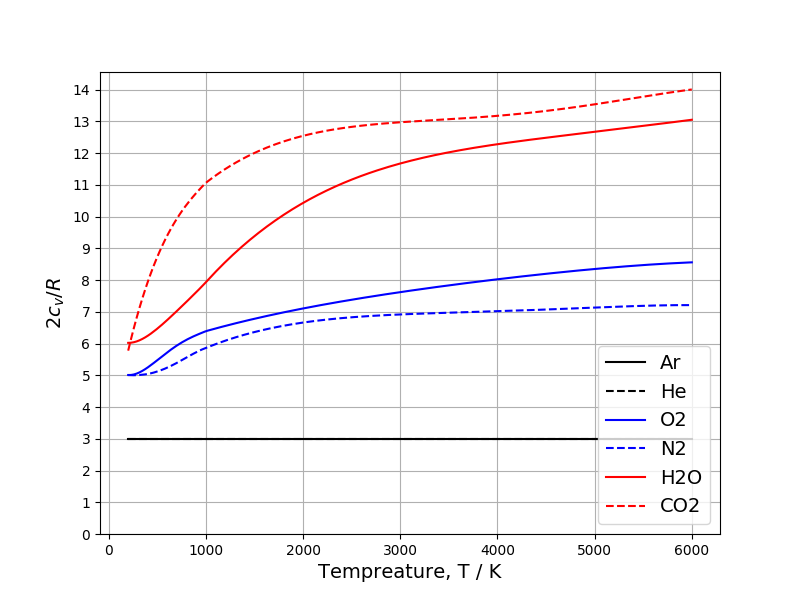
\includegraphics[width=0.97\textwidth]{figures/dof}
\caption{Approximate mean active degrees of freedom in selected ideal gas models}\label{fig:dof}
\end{figure}

For H$_2$O, rigid motion means six degrees of freedom: three coordinates of translation and three axes of rotation.  For diatomic molecules like O$_2$ and N$_2$, however, their symmetry robs them of one of their axes of rotation, so they only exhibit five degrees of freedom at low temperatures.  Since CO$_2$ is also an axisymmetric molecule, it can be seen asymptotically approaching 5 at low temperatures as well.

\subsection{Entropy and enthalpy revisited}

Recall from Section \ref{sec:intro:s} that the entropy of any substance changes like
\begin{align}
T \d s = \d h - v \d p\nonumber.
\end{align}
For the ideal gas, this can be simplified by substituting $R T / p$ for $v$ and integrating to obtain
\begin{align}
s - s_0 = \int c_p(T)\frac{\d T}{T} - R \ln \left( \frac{p}{p^\circ} \right)\label{eqn:ig:s}.
\end{align}
when $p^\circ$ is a reference pressure.  For a perfect gas,
\begin{align}
s - s_0 = c_p \ln\left( \frac{T}{T_0} \right) - R \ln\left( \frac{p}{p^\circ} \right)\label{eqn:pg:s}.
\end{align}
when $T_0$ is a reference temperature.

Evaluating the pressure portion of (\ref{eqn:pg:s}) is straightforward, but it will be seen below that the temperature dependence is more nuanced.  For that reason, it is often treated alone,
\begin{align}
s^\circ(T) = s_0 + \int c_p(T) \frac{\d T}{T},
\end{align}
where $s^\circ$ is the entropy at the reference pressure, $p^\circ$.

An identical approach can be taken for enthalpy, but with an even simpler result.  
\begin{align}
h - h_0 = \int c_p(T) \d T \label{eqn:ig:h}
\end{align}
For a perfect gas,
\begin{align}
h - h_0 = c_p \left(T - T_0\right). \label{eqn:pg:h}
\end{align}

In the NIST-JANAF tables, the specific heat is calculated theoretically from the molecular and atomic structure of each atom, but specific heat is also readily validated by calorimetry.  Entropy's integration constant, $s_0$, is chosen so the values agree with absolute calculations for the species entropy from Boltzmann's statistical model for entropy.  Since no such model exists for enthalpy, $h_0$ is determined by a separate approach described in Section \ref{sec:hf}.

The models in the \texttt{ig} and \texttt{ig2} classes use systems of coefficients to form piece-wise polynomials for $c_p(T)$ instead of using the detailed models recorded in the NIST-JANAF tables.  These are ideal for computational codes because they give good numerical performance, but they are not valid down to the low temperatures included by the original tables.

\subsection{Other properties}

Once $c_p(T)$ is well defined, it is also possible to evaluate internal energy,
\begin{align}
e(T) = h(T) - RT,\label{eqn:ig:e}
\end{align}
constant-volume specific heat,
\begin{align}
c_v(T) = c_p(T) - R,\label{eqn:ig:cv}
\end{align}
specific heat ratio,
\begin{align}
\gamma(T) = \frac{c_p(T)}{c_p(T) - R},\label{eqn:ig:cp}
\end{align}
speed of sound
\begin{align}
a(T) = \sqrt{\gamma(T) R T},\label{eqn:ig:a}
\end{align}
and others.

\subsection{Enthalpy of formation}\label{sec:ig:hf}

When a substance is formed either by nuclear, chemical or phase change, energy is nearly always released or consumed.  This energy is accounted for by a property called the \emph{enthalpy of formation}.  It is the energy required to form a substance, so exothermic reactions have negative enthalpies of formation.  The ideal gas data on which \PM's ideal gas classes do not consider nuclear reactions; only chemical reactions and phase changes.  

One might imagine a reactor with a mixture of reactants flowing in and a mixture of products flowing out.  In the simplest case, we should imagine the products to be made entirely of the substance we wish to study, so the reactants will be only those that are absolutely necessary for forming it and in the correct proportions.
\begin{align}
a \mathrm{A}+ b \mathrm{B} + \ldots \rightarrow \mathrm{A}_a \mathrm{B}_b \ldots
\end{align}

Many such chemical reactions release or consume vast amounts of energy.  Usually, this results in cooling or heating of the substance as it changes.  When heat and work are neither added nor removed from the system, an energy balance mandates an isenthalic process,
\begin{align}
h_\mathrm{reactants} &= h_\mathrm{products}\nonumber\\
a \overline{h}_\mathrm{A} + b \overline{h}_\mathrm{B} + \ldots &= \overline{h}_{\mathrm{A}_a \mathrm{B}_b \ldots}
\end{align}
when $\overline{h}$ is enthalpy in molar units.

This result is often counter intuitive.  Since ideal gas enthalpy is only a function of temperature, it seems like an isenthalpic process should also be isothermal.  However, when chemical or phase changes take place, the enthalpy curves of the products and reactants can be dramatically different.  

Fig. \ref{fig:hf} shows enthalpy curves for a hypothetical set of reactants and products.  Not only may the two have dissimilar slopes, but the curves may have large offsets separating them.  When the process is isenthalpic, these offsets cause temperature changes shown in red.  In the case shown, the reactants have higher enthalpy than the products, so the additional energy is absorbed thermally by the products, causing an increase in temperature.  On a molecular level, the effect is like allowing two magnetic marbles to roll near one another on a flat table.  Even if neither has much velocity to begin with, after they collide, they will be sent off quickly spinning and rolling.  The same happens in an exothermic reaction.

\begin{figure}
\centering
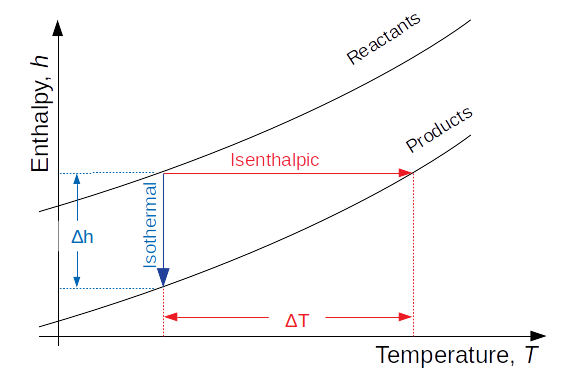
\includegraphics[width=.97\linewidth]{figures/hf}
\caption{Isenthalpic and isothermal reactions on an h-T diagram.}\label{fig:hf}
\end{figure}

If the hypothetical reactor were modified to add or extract heat so that the temperature of the reaction were constant, the process would adopt the vertical blue line instead.  In an isothermal reaction, the amount of thermal energy exhibited by the substance is constant, so any release or consumption of heat will have come from a chemical reaction (including a change in the substance's active degrees of freedom, $f$).  Therefore, the change in enthalpy between the two curves is the enthalpy consumed by the chemical reaction reaction.  

In the diagram, the enthalpy is seen decreasing in order to maintain the temperature, so heat was removed, and the reaction is called exothermic.  For such a reaction, the energy balance would be
\begin{align}
a \overline{h}_\mathrm{A} + b \overline{h}_\mathrm{B} + \ldots + \Delta h &= \overline{h}_{\mathrm{A}_a \mathrm{B}_b \ldots}
\end{align}
Here, the change in enthalpy, $\Delta h$, is positive when energy is added to maintain a constant temperature throughout the reaction, so in the exothermic reaction depicted in fig. \ref{fig:hf}, $\Delta h$ would be negative.  In general $\Delta h$ is also a function of temperature because the properties of the two gas mixtures are not parallel.

The value of $\Delta h(T)$ also depends on which reactants are selected to form the product.  For example, one might select atomic oxygen and atomic hydrogen to form water, but it would be just as valid to chose the more common diatomic hydrogen and oxygen.  These two reactions would exhibit different $\Delta h$ values because the energies of the starting substances are different.  If one wishes to establish a value for $\Delta h$ that is clearly defined and indicates the energy required to form the substance, it is necessary to specify a standard set of ``reference'' substances, relative to which all other substances are derived.

Every element is given exactly one {\bf reference substance}, which may include phase changes (like in the case of the metals).  The enthalpy of formation for the reference substance is arbitrarily declared to be zero at all temperatures, since it is imagined to be a fundamental building block from which compounds are built.

The \emph{enthalpy of formation}, $\Delta_f h$, is the energy consumed by the reaction when all of the reactants are reference substances in the proper proportions to produce the product.

Many of the reference substances are atomic gases or pure liquids and crystals (like argon and aluminum).  Others are selected to be diatomic gases because of their abundance (like hydrogen, oxygen, and nitrogen).

\subsection{Properties of mixtures}\label{sec:ig:mix}

The discussion so far has applied only to properties of pure ideal gases.  The composition of a gas mixture is conventionally defined in either mass or molar quantities of the constituent pure gases.  In this section, we establish methods by which properties can be calculated from the properties of the components.  

In extensive units, a volume, $V$, might contain many individual gas species, each with total mass, $m_i$, or total mole count, $N_i$.  They are related by the pure gas's molecular weight,
\begin{align}
m_i = W_i N_i.
\end{align}

{\bf Mass and mole fractions} are the fractions of a gas composed of a single pure substance. The total mass and count of gas in the volume is merely the sum of all the constituents, $m = \sum m_i$, and $N = \sum N_i$.  These let us more conveniently express the composition in mass and mole fractions, respectively,
\begin{subequations}
\begin{align}
y_i &\equiv \frac{m_i}{\sum m_k}\\
\chi_i &= \equiv \frac{N_i}{\sum N_k}.
\end{align}
\end{subequations}
Note that the fractional quantities, $y_i$ and $\chi_i$, are not dependent on the choice of units for mass or mole count.  Observe that, by definition, $\sum y_i = \sum \chi_i = 1$.

{\bf Mixture density} is the total mass or mole count of all species divided by the volume they occupy.  
\begin{subequations}
\begin{align}
\rho &\equiv \frac{\sum m_i}{V}\\
\overline{\rho} &\equiv \frac{\sum N_i}{V}
\end{align}
\end{subequations}
If $\rho_i$ and $\overline{\rho}_i$ were the densities of constituent $i$ at the same temperature and pressure as the total mixture, then it is important to emphasize that $m_i / V$  and $N_i / V$ are \emph{not} $\rho_i$ and $\overline{\rho}_i$.  That question is addressed below.

{\bf Molecular weight} of a gas mixture has the same definition as the molecular weight of a pure gas; it is the mass per mole count of total gas.  It can be calculated from the constituent molecular weights using either mole fractions or mass fractions,
\begin{subequations}
\begin{align}
W &\equiv \frac{\sum m_i}{\sum N_j}\\
 &= \frac{\sum N_i W_i}{\sum N_j}\nonumber\\
 &= \sum \chi_i W_i\label{eqn:w:x}\\
 &= \frac{\sum m_i}{\sum m_j / W_j}\nonumber\\\
 &= \left(\sum \frac{y_j}{W_j} \right)^{-1}.\label{eqn:w:y}
\end{align}
\end{subequations}

{\bf Partial pressure}, $p_i$, is the pressure force exerted on a surface due only to collisions of a single constituent, $i$.  Section \ref{sec:iglaw} will help understand what is meant by this idea.  It is the pressure force that would be measured if all other constituent gases were removed.  
\begin{align}
p_i &\equiv \frac{N_i}{V} R_u T \nonumber\\
 &= \chi_i \frac{N}{V} R_u T \nonumber\\
 &= \chi_i \overline{\rho} R_u T
\end{align}

The same pressure may be calculated from mass fraction,
\begin{align}
p_i &= \frac{N_i}{V} R_u T \nonumber\\
 &= \frac{m_i}{W_i V} \rho R_u T \nonumber\\
 &= y_i \rho R_i T
\end{align}
The ideal gas constant, $R_i$, is the mass-based gas constant for only that constituent, $R_i = R_u / W_i$.

{\bf Total pressure}, $p$, is the pressure force actually experienced by a surface due to all of the constituent gases.  By definition, 
\begin{align}
p &= \sum p_i \nonumber\\
 &= \overline{\rho} R_u T
\end{align}
Observe, also, that 
\begin{align}
\chi_i = \frac{p_i}{p}.
\end{align}

The total pressure can also be calculated in terms of mass density.  Using (\ref{eqn:w:y}),
\begin{align}
p &= \sum p_i \nonumber\\
 &= \sum y_i \rho R_i T\nonumber\\
 &= \sum \frac{y_i}{W_i} \rho R_u T\nonumber\\
 &= \rho R T.
\end{align}
The total mixture gas constant appears naturally.

{\bf The mixture gas constant}, $R$, appears naturally when calculating total pressure from total mass density, and it is calculated in precisely the same way as a pure gas constant, but the mixture molecular weight is used instead,
\begin{subequations}
\begin{align}
R &\equiv \frac{R_u}{W}\\
 &= \frac{R_u}{\sum \chi_i W_i}\nonumber\\
 &= \left( \frac{\chi_i}{R_i} \right)^{-1}\\
 &= R_u \sum \frac{y_i}{W_i}\nonumber\\
 &= \sum y_i R_i
\end{align}
\end{subequations}

{\bf Densities} can be calculated from the same properties of the component species using the ideal gas law.  For mass density,
\begin{subequations}
\begin{align}
\rho &= \frac{p}{R T}\nonumber\\
 &= \frac{p}{\sum y_i R_i T}\nonumber\\
 &= \left(\sum \frac{y_i}{\rho_i(T,p)} \right)^{-1}\\
 &= \frac{p}{\left(\sum \chi_i / R_i\right)^{-1} T}\nonumber\\
 &= \sum \chi_i \rho_i(T,p)
\end{align}
\end{subequations}

For molar density, no such complexity is needed, since the universal gas constant is the same for all gases,
\begin{align}
\overline{\rho} &= \frac{p}{R_u T}\nonumber
\end{align}

{\bf Internal energy, enthalpy, entropy, and other bulk properties} are merely the sum of all the values contributed by each of the constituent gases.  By definition in an ideal gas, the presence of other gases do not affect the behavior of each of the pure constituents.  Therefore, a bulk property may be calculated from the properties of the pure substances under equivalent temperature and pressure,
\begin{align}
\left(\sum m_j\right) \phi(T,p) &= \sum m_i \phi_i(T,p)\nonumber\\
\left(\sum N_j \right) \overline{\phi}(T,p) &= \sum N_i \overline{\phi}_i(T,p)\nonumber
\end{align}
Therefore, 
\begin{align}
\phi(T,p) &= \sum y_i \phi_i(T,p)\nonumber\\
\overline{\phi}(T,p) &= \sum \chi_i(T,p) \overline{\phi}_i\nonumber
\end{align}
This is hardly a proof, but it is sufficient for the scope of this document to assert that it is true for bulk properties.

This identity may be applied to internal energy, enthalpy, entropy, and all the properties derived from them, so
\begin{subequations}
\begin{align}
e(T) &= \sum y_i e_i(T)\\
h(T) &= \sum y_i h_i(T)\\
s(T,p) &= \sum y_i s_i(T,p)
\end{align}
\end{subequations}
and
\begin{subequations}
\begin{align}
\overline{e}(T) &= \sum \chi_i \overline{e}_i(T)\\
\overline{h}(T) &= \sum \chi_i \overline{h}_i(T)\\
\overline{s}(T,p) &= \sum \chi_i \overline{s}_i(T,p).
\end{align}
\end{subequations}


\section{The ideal gas collection}

There are several classes that implement various data models for ideal gas properties.  Their interfaces are all standardized so that very little difference should be apparent to the user, except that the ideal gas mixture class has some extra methods associated with its composition.

All property methods accept any two of temperature, density, or pressure to specify the state.

\subsection{The Shomate equation: \texttt{ig}}\label{sec:ig:ig}

\PM's \texttt{ig1} class is built on the Shomate equation for constant-pressure specific heat $c_p$.  This is the formulation used by the NIST webbook \cite{nist:webbook}.  Despite the wise range of substances represented, it has the advantage of using a simple standard piece-wise formulation for specific heat.  However, it does suffer from certain limitations.

The Shomate equation takes the form
\begin{align}
\theta &= \frac{T}{T_s}\\
c_p(t) &= c_0 + c_1 \theta + c_2 \theta^2 + c_3 \theta^3 + \frac{c_4}{\theta^2},
\end{align}
where the scaling temperature, $T_s$ is 1000K for all species.  The decision to scale the temperature by a large value has the effect of scaling $\tau$ so that it will not be much larger than 5 or 6.  That helps reduce numerical errors in high-order polynomials.

Because of its simplicity, the Shomate equations lack the degrees of freedom to express specific heat over wide ranges, so data are usually given in piece-wise formulations.  For example, tungsten dioxide (WO$_2$), has a set of coefficients for $298\mathrm{K} \le T < 1100\mathrm{K}$ and $1100\mathrm{K} \le T \le 6000\mathrm{K}$.

The enthalpy can be explicitly calculated from (\ref{eqn:ig:enthalpy}),
\begin{align}
h(T) &= h_0 + \int c_p(T) \d T \nonumber\\
 &= h_0 + T_s \int c_p(\theta) \d \theta \nonumber\\
 &= T_s \left(c_0 \theta + \frac{c_1}{2} \theta^2 + \frac{c_2}{3} \theta^3 + \frac{c_3}{4} \theta^4 - \frac{c_4}{\theta} + c_5 \right).
\end{align}
It is important to emphasize that $h_0$ is not the same as the enthalpy of formation, $\Delta h^\circ_f$.  Instead, it is merely an integration constant, which can be alternately expressed as a new coefficient, $c_5$.

Because of the temperature term in the denominator, no multiple of $T_s$ appears in entropy when the integration is changed to $\theta$,
\begin{align}
s^\circ(T) &= s_0 + \int \frac{c_p(T)}{T}\d T\nonumber\\
 &= s_0 + \int \frac{c_p(\theta)}{\theta}\d \tau\nonumber\\
 &= c_0 \ln \theta + c_1 \theta + \frac{c_2}{2} \theta^2 + \frac{c_3}{3} \theta^3 -\frac{c_4}{2\theta^2} + c_6\\
s(T,p) &= s^\circ(T) - R \ln \left( \frac{p}{p^\circ} \right)\nonumber
\end{align}
Just like in the enthalpy integral, a new coefficient, $c_6$, has been introduced to represent the integration constant.

Internal energy is readily calculated from the definition of enthalpy in (\ref{eqn:enthalpy}),
\begin{align}
e(T) &= h(T) - RT
\end{align}
There is a similarly simple relationship to determine constant-volume specific heat and specific heat ratio,
\begin{align}
c_v(T) &= c_p(T) - R\\
\gamma(T) &= \frac{c_p(T)}{c_p(T)-R}
\end{align}

Table \ref{tab:class:ig} lists the data elements that define the \texttt{ig} class.  For more information on how \texttt{.hpd} files are stored, see Section \ref{sec:data}.  Most of the essential data elements are self explanatory, but the coefficients and temperature limits must have compatible sizes.  Even though the \texttt{ig} class only uses seven coefficients, there are eight provided in the NIST data sets.  If there are $N$ sets of coefficients defined over $N$ temperature ranges, there must be $N$ arrays of eight coefficients and $N+1$ temperature limit values.
5
For example, in a data set with two temperature ranges, the following would define a data set valid between \texttt{<T0>} and \texttt{<T2>}, and the transition between the two piece-wise data sets is at \texttt{<T1>}.
\begin{lstlisting}[language=Python]
"Tlim":[<T0>, <T1>, <T2>]
"C":[
  [ <c0>, <c1>, <c2>, <c3>, <c4>, <c5>, <c6>, <c7> ],
  [ <c0>, <c1>, <c2>, <c3>, <c4>, <c5>, <c6>, <c7> ],
]
\end{lstlisting}

\begin{table}
\centering
\caption{HPD data file elements for the \texttt{ig} class}\label{tab:class:ig}
\begin{tabular}{|ccp{2.5in}|}
\hline
Name & Type & Description\\
\hline
\texttt{id} & \texttt{str} & Unique substance identifier string\\
\texttt{class} & \texttt{='ig'} & Class identifier string\\
\texttt{doc} & \texttt{str} & Documentation string\\
\hline
\texttt{atoms} & \texttt{dict} & Keys are elemental atoms, and values are their integer quantities in the substance.\\
\texttt{mw} & \texttt{float} & The molecular weight.\\
\texttt{Tlim} & \texttt{list} & A sorted list of $N+1$ floating point temperatures.  Middle values define the boundaries between piece-wise coefficient ranges.  High and low values define the limits of the model.\\
\texttt{C} & nested \texttt{list} & The value, $C[i][j]$, corresponds to coefficient $c_j$ in the temperature interval \texttt{Tlim[i]} to \texttt{Tlim[i+1]}.\\
\hline
\texttt{TAB} & nested \texttt{list} & Optional table of truth values published by NIST used for validation\\
\hline
\end{tabular}
\end{table}


\subsection{The NASA polynomial: \texttt{ig2}}\label{sec:ig:ig2}

The so-called ``NASA polynomials'' are a piece-wise empirical formulation to the specific heat of an ideal gas.  They predate the latest formulation of the NIST-JANAF tables, and are even used for reference.  Unlike the Shomate equation, there is no $1/t^2$ term, there is no attempt to scale temperature prior to evaluating the polynomial, and properties are scaled with respect to the ideal gas constant.

\begin{align}
c_p(T) = R\left(c_0 + c_1 T + c_2 T^2 + c_3 T^3 + c_4 T^4\right)
\end{align}

There are nearly identical formulations for enthalpy,
\begin{align}
h(T) = R \left(c_0 T + \frac{c_1}{2} T^2 + \frac{c_2}{3} T^3 + \frac{c_3}{4} T^4 + \frac{c_4}{5}T^5 + c_5 \right),
\end{align}
and entropy
\begin{align}
s^\circ(T) = R \left(c_0 \ln(T) + c_1 T + \frac{c_2}{2} T^2 + \frac{c_3}{3} T^3 + \frac{c_4}{4} T^4 + c_6\right).
\end{align}
Here, just as in the Shomate equations, $c_5$ and $c_6$ are introduced as integration constants in enthalpy and entropy.

Internal energy is readily calculated from the definition of enthalpy in (\ref{eqn:enthalpy}),
\begin{align}
e(T) &= h(T) - RT\nonumber\\
\end{align}
There is a similarly simple relationship to determine constant-volume specific heat and specific heat ratio,
\begin{align}
c_v(T) &= c_p(T) - R\\
\gamma(T) &= \frac{c_p(T)}{c_p(T)-R}
\end{align}

There is some overlap in the species offered by the two classes.  A mild preference has been given to the older NASA polynomials for two reasons:
\begin{itemize}
\item Most of the NASA models have wider ranges of validity than the Shomate models.
\item Some of the Shomate data have been found to suffer from discontinuity errors at the piecewise boundaries.
\end{itemize}
Otherwise, the two have been found to be sufficiently equivalent that most users will not find a reason to wonder.

Table \ref{tab:class:ig2} lists the data elements that define the \texttt{ig2} class.  For more information on how \texttt{.hpd} files are stored, see Section \ref{sec:data}.  Most of the essential data elements are self explanatory, but the coefficients and temperature limits must have compatible sizes.  Even though the \texttt{ig2} class only uses seven coefficients, there are eight provided in the NIST data sets.  If there are $N$ sets of coefficients defined over $N$ temperature ranges, there must be $N$ arrays of eight coefficients and $N+1$ temperature limit values.

For example, in a data set with two temperature ranges, the following would define a data set valid between \texttt{<T0>} and \texttt{<T2>}, and the transition between the two piece-wise data sets is at \texttt{<T1>}.
\begin{lstlisting}[language=Python]
"Tlim":[<T0>, <T1>, <T2>]
"C":[
  [<c0>, <c1>, <c2>, <c3>, <c4>, <c5>, <c6>, <c7>],
  [<c0>, <c1>, <c2>, <c3>, <c4>, <c5>, <c6>, <c7>],
]
\end{lstlisting}

\begin{table}
\centering
\caption{HPD data file elements for the \texttt{ig2} class}\label{tab:class:ig2}
\begin{tabular}{|ccp{2.5in}|}
\hline
Name & Type & Description\\
\hline
\texttt{id} & \texttt{str} & Unique substance identifier string\\
\texttt{class} & \texttt{='ig2'} & Class identifier string\\
\texttt{doc} & \texttt{str} & Documentation string\\
\hline
\texttt{atoms} & \texttt{dict} & Keys are elemental atoms, and values are their integer quantities in the substance.\\
\texttt{pref} & \texttt{float} & Reference pressure in Pascals\\
\texttt{mw} & \texttt{float} & The molecular weight.\\
\texttt{Tlim} & \texttt{list} & A sorted list of $N+1$ floating point temperatures: Middle values define the boundaries between piece-wise coefficient ranges.  High and low values define the limits of the model.\\
\texttt{C} & nested \texttt{list} & The value, $C[i][j]$, corresponds to coefficient $c_j$ in the temperature interval \texttt{Tlim[i]} to \texttt{Tlim[i+1]}.\\
\hline
\end{tabular}
\end{table}

\subsection{The ideal gas mixture: \texttt{igmix}}\label{sec:ig:igmix}

The \PM\ ideal gas mixture class defines methods to calculate properties of a static mixture of ideal gases.  For improved computational efficiency, properties like the mixture molecular weight, mole fractions, and mass fractions, are calculated ahead of time and stored in class instances for later use.

Section \ref{sec:ig:mix} already shows how properties of a mixture can be calculated from the properties of the constituent gases.  The implementation of all but entropy is quite straightforward.  In all of the ideal gas codes, the entropy at the reference pressure, $s^\circ$, is calculated in a separate efficient internal method.  For that reason, the \texttt{igmix} class calls on these methods directly and then treats the pressure dependence separately.

When calculating in molar units,
\begin{align*}
\overline{s}(T,p) &= \sum \chi_i\ \overline{s}^\circ_i(T) - \sum \chi_i R_u \ln\left(\frac{p}{p^\circ_i}\right)
\end{align*}
Note that in this formulation, the constituents are not required to have the same reference pressure.  This can be dealt with by calculating an effective mixture reference pressure.  
\begin{align*}
\sum \chi_i \ln\left(\frac{p}{p^\circ_i}\right) &= \sum \chi_i \left( \ln p - \ln p^\circ_i \right)\\
&= \ln p - \sum \chi_i \ln p^\circ_i\\
&= \ln \left(\frac{p}{p^\circ_{mix}}\right)
\end{align*}
when
\begin{align}
p^\circ_{mix} = \exp\left(\sum \chi_i \ln p^\circ_i \right).
\end{align}
This is a log-weighted average of the constituent reference pressures.  In the event that they are all the same, the mixture reference pressure is also the same.

It is less direct, but the same equivalent reference pressure can be derived from the mass-unit properties as well.  So,
\begin{subequations}
\begin{align}
s(T,p) &= \sum \chi_i \overline{s}^\circ_i(T) - R \ln\left(\frac{p}{p^\circ_{mix}}\right)\\
\overline{s}(T,p) &= \sum \chi_i \overline{s}^\circ_i(T) - R_u \ln\left(\frac{p}{p^\circ_{mix}}\right)
\end{align}
\end{subequations}

\begin{table}
\centering
\caption{HPD data file elements for the \texttt{igmix} class}\label{tab:class:igmix}
\begin{tabular}{|ccp{2.5in}|}
\hline
Name & Type & Description\\
\hline
\texttt{id} & \texttt{str} & Unique substance identifier string\\
\texttt{class} & \texttt{='igmix'} & Class identifier string\\
\texttt{doc} & \texttt{str} & Documentation string\\
\hline
\texttt{bymass} & \texttt{bool} & Indicates whether contents are listed by mass or by mole count\\
\texttt{contents} & \texttt{dict} & Specifies the mixture composition: Keys are pure ideal gas id strings, values are quantities.  The quantities will be normalized after load, so they do not need to add to one.\\
\hline
\end{tabular}
\end{table}

